% !TEX options=--shell-escape
\documentclass[a4paper, 11pt]{article}
\usepackage[utf8]{inputenc}
\usepackage[left=1in,right=1in,bottom=0.8in]{geometry}
\usepackage{enumitem}
\usepackage{graphicx}
\graphicspath{ {Figures/} }
\usepackage{float}
\usepackage[labelfont=bf]{caption}
\usepackage{fixltx2e}
\usepackage{caption}
\usepackage{amsmath}
\usepackage{capt-of}
\usepackage{minted}
\usepackage{tabu}
\usepackage{pgf}
\usepackage{tikz}
\usetikzlibrary{arrows,automata}

\let\svthefootnote\thefootnote


\title{\bf Experiment 4\\\vspace*{2mm} Debouncing a switch}
\author{\it Amit Kumar | 16D070034}
\date{March 27, 2018}

\begin{document}
\maketitle
\section*{Overview}
In this experiment, we implemented a Finite state machine to be used as a debouncing circuit to clean up the output of the push-button/switch as they take time to settle (typically a few milli-seconds) and during this settling period, the output may touch 0 and 1 several times which we wanted to prevent .
 
\noindent So, we implemented it in VHDL which  was  compiled  on  Quartus  Prime,  and  simulated using  ModelSim  whichwas then uploaded to theKrypton v1.15M1270ZT144C5N CPLD-based board via svf file and urjtag and tested using a simple switch and led with oscilloscope.

\section{Setup}
% The english alphabet is represented by 5 bits ($\lceil log_2(26) \rceil$), and a bit each for \emph{clock} and \emph{reset} results in 7 input bits which were encoded by converting alphabet position (1-26) to 5-bit binary, for simplicity. I have implemented recognizer for each string individually using FSM mealy model then combined all entities to detect the presence of all four strings .
First , We implemeted a counter to generate a clock of 100 Hz from 50MHz and then ysed that to implement debouncing FSM . All subparts are explained below :

\subsection{Counter}

Since CPLD has an inbuilt clock port of frequency 50MHz .So in order to use that clock for our deboucing circuit, I have made a counter to generate a lower frequency 100M Hz clock to check at intervals of 10ms.
Following the code of counter to genarate $f/2$ if input is $f$ : \\
\inputminted[linenos]{vhdl}{counter.vhd}

\noindent Further, I have cascades 19 $f/2$ counters to genarate clock of frequency $f/2^19$ for our purpose :
\inputminted[linenos]{vhdl}{counter2.vhd}

\subsection{Debouncing FSM}

Using this 100Hz clock, I have designed a debouncing FSM which has a single
input from the switch/push-button (and also a reset), and a single
output which produces clean switching between 0 and 1 using two input gates, inverters and D flip-flops.

{\bf FSM Logic :} \\
The switch output is checked every 10ms, and the output of the finite-state machine is 1 (respectively, 0) if the last two values that were checked are 1 (respectively, 0).

% \begin{figure}[H]
% \centering
% \includegraphics[width=12cm]{trans.jpg}
% \caption{Automata Representation for debouncing FSM}
% \end{figure} 

Using the above state representation, the encoding has been done as shown below.
\begin{center}
\begin{tabular}{| c | c | c |}
\hline
\bf State & \bf $q_0$ & \bf $q_1$\\
\hline
$S_0$ & 0 & 0 \\
$S_1$ & 0 & 1 \\
$S_2$ & 1 & 0 \\
\hline
\end{tabular}
\end{center}

Below is the transition table with input 'x' and putput 'y'
\begin{center}
\begin{tabular}{| c | c | c | c | c | c |}
\hline
\bf x & \bf $q_0$ & \bf $q_1$ & \bf $nq_0$ & \bf $nq_1$ & \bf y \\
\hline
0 & 0 & 0 & 0 & 0 & 0 \\
0 & 0 & 1 & 0 & 1 & 0\\
0 & 1 & 0 & 0 & 0 & 0 \\
0 & 1 & 1 & 1 & 0 & 1 \\
1 & 0 & 0 & 0 & 1 & 1 \\
1 & 0 & 1 & 1 & 0 & 1 \\
\hline
\end{tabular}
\end{center}

VHDL code of debouncing FSM :\\
\inputminted[linenos]{vhdl}{debounce.vhd}

\noindent Final Integration of our counter and Debouncing FSM :
\inputminted[linenos]{vhdl}{DUT.vhd}




\section{Observations}
After implementing the design in code, the next major part is to simulate and test the code for a set of inputs. RTL simulation was performed on the machine to validate the implementation.


\begin{figure}[H]
\centering
\includegraphics[width=18cm]{final.png}
\caption{Working of counter for generating 100 $Hz$}
\end{figure}

\begin{figure}[H]
\centering
\includegraphics[width=18cm]{deb.png}
\caption{Simulation of debouncer for a particular test case}
\end{figure}


\section{DSO Testing}

We have tested the logic using the RTL simulations,then done pin planning and burned svf file of code on the Krypton board using urjtag . Next, we need to check that the code is actually running as it is expected to, on the board.Hence we connected an additional LED and switch and observed on oscilloscope.


\begin{figure}[H]
\centering
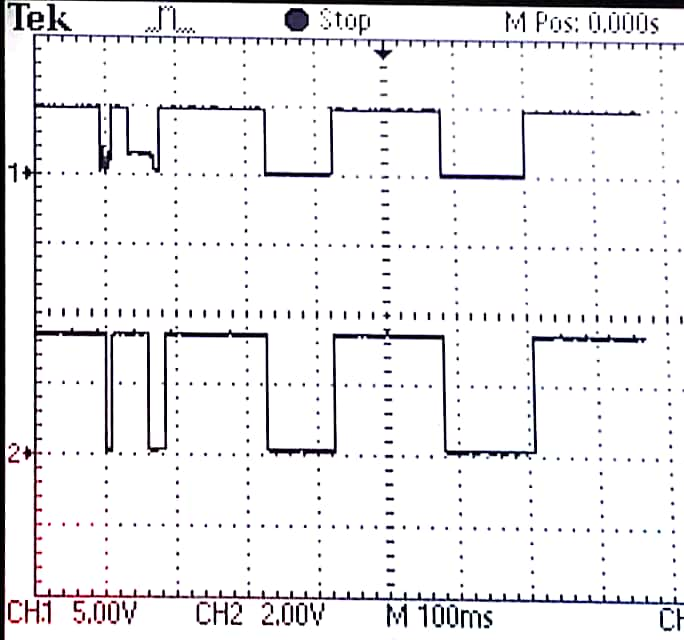
\includegraphics[width=12cm]{dso.jpg}
\caption{Debounced output}
\end{figure}
P.S: In above figure , Initial is not a bounce , it appears as time scale is 100 ms and input was 0 for past 20ms .

\end{document}
